\documentclass[a0paper,portrait]{baposter}

\usepackage{wrapfig}
\usepackage{lmodern}
\usepackage{amsmath}
\usepackage{enumitem}
\usepackage{xcolor}

\usepackage[utf8]{inputenc} %unicode support
\usepackage[T1]{fontenc}


\selectcolormodel{cmyk}

\graphicspath{{figures/}} % Directory in which figures are stored


\newcommand{\compresslist}{%
\setlength{\itemsep}{0pt}%
\setlength{\parskip}{1pt}%
\setlength{\parsep}{0pt}%
}

\newenvironment{boenumerate}
  {\begin{enumerate}\renewcommand\labelenumi{\textbf\theenumi.}}
  {\end{enumerate}}



\begin{document}

\definecolor{darkblue}{rgb}{0.1,0.2,1.0}
\definecolor{lightblue}{rgb}{0.2,0.4,0.8}

\begin{poster}
{
grid=false,
headerborder=open, % Adds a border around the header of content boxes
colspacing=1em, % Column spacing
bgColorOne=white, % Background color for the gradient on the left side of the poster
bgColorTwo=white, % Background color for the gradient on the right side of the poster
borderColor=darkblue, % Border color
headerColorOne=lightblue, % Background color for the header in the content boxes (left side)
headerColorTwo=lightblue, % Background color for the header in the content boxes (right side)
headerFontColor=white, % Text color for the header text in the content boxes
boxColorOne=white, % Background color of the content boxes
textborder=rounded, %rectangle, % Format of the border around content boxes, can be: none, bars, coils, triangles, rectangle, rounded, roundedsmall, roundedright or faded
eyecatcher=false, % Set to false for ignoring the left logo in the title and move the title left
headerheight=0.11\textheight, % Height of the header
headershape=rounded, % Specify the rounded corner in the content box headers, can be: rectangle, small-rounded, roundedright, roundedleft or rounded
headershade=plain,
headerfont=\Large\textsf, % Large, bold and sans serif font in the headers of content boxes
%textfont={\setlength{\parindent}{1.5em}}, % Uncomment for paragraph indentation
linewidth=2pt % Width of the border lines around content boxes
}
{}
%
%----------------------------------------------------------------------------------------
%	TITLE AND AUTHOR NAME
%----------------------------------------------------------------------------------------
%
{
\textsf %Sans Serif
{Comparison of different techniques for image augmentation.
}
} % Poster title
% {\vspace{1em} Marta Stepniewska, Pawel Siedlecki\\ % Author names
% {\small \vspace{0.7em} Department of Bioinformatics, Institute of Biochemistry and Biophysics, PAS, Warsaw, Pawinskiego 5a}} % Author email addresses
{\sf\vspace{0.5em}\\
Ralph Lesch and Joshua Heipel
\vspace{0.1em}\\
\small{University of Freiburg, Department of Computer Science, Deep Learning Bachelor Project
\vspace{0.2em}\\
joshua.heipel@gmx.de}
}
%{
\includegraphics{logo}} % University/lab logo


\headerbox{1. Introduction}{name=introduction,column=0,row=0, span=3}{
Convolutional Neural Networks (CNNs) have become a major aproach for the task of Semantic Segmentation and are nowadays used widely over many different fields of applications. Although for some use cases large datasets with thousands of (manually) labeled images have been published (such as CamVid or CityScape in the context of city traffic), in many situations appropriate training data still remains sparse. As a consequence Deep Neural Networks with lots of trainable parameters tend to overfit small and monotonous datasets while generating poor predictions for new (unseen) observations. In order to improve generalization of such CNNs existing training data can be extended by employing different techniques of image augmentation. 
}


\headerbox{2. Architecture}{name=architecture,column=0,below=introduction,span=1}{

In our case study we use a hierarchical encoder-decoder network with skip connections (CNN of exercise 3) to compare different settings:

\begin{enumerate}[label={(\arabic*)}]
    \item \textbf{No Augmentation}
    \item \textbf{Shape Augmentation} by applying different geometric transformation and dropouts (Horizontal Flip, Scaling, Crop and Padding, rectangular Cutouts)
    \item \textbf{Color Augmentation} by varying the intensity values (Adjustment of Brightness and Contrast, Color shifts)
    \item \textbf{Shape and Color Augmentation}
\end{enumerate} 



\begin{center}
%    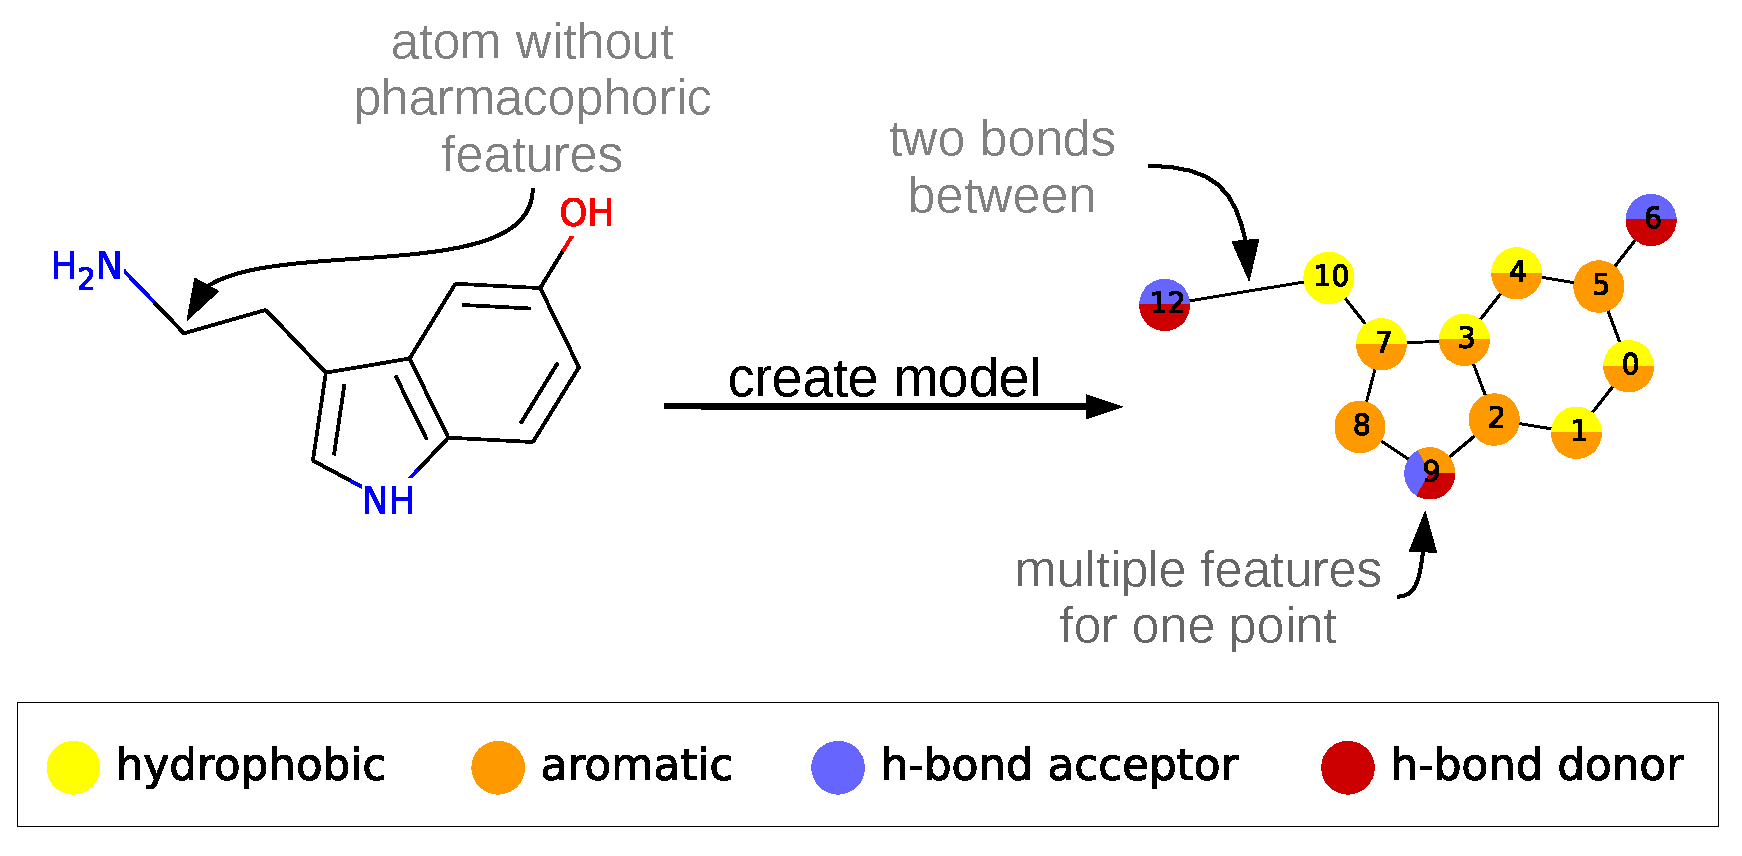
\includegraphics[width=\linewidth]{phar}
\end{center}
%\vspace{-2pt}
}


\headerbox{3. Training}{name=training,column=0,below=architecture,span=1}{

The network is trained on CamVid dataset, which contains ???? different labeled images. To allow for a fair comparison between the 4 different configurations, we use the same hyperparameters (namely the total amount of iterations and batch size) for all types of augmentation. Batches are created by sampling images from the original dataset with pseudo-random numbers and then applying augmentations for setting (2) - (4) on 90\% of the images. To facilitate multiple independent modifications $A_k$ (e.g. cropping and flipping an image) we implemented our own probabilistic framework based on the principle of inclusion and exclusion, where:
%\[P(A_i \cup A_j) = P(A_i) + P(A_j) - P(A_i \cap A_j)\] \[= 2\cdot P(A_i) - P(A_i)^2\] or in more general form: 
\[P\left(\bigcup_{k=1}^{n} A_k\right) = \sum_{k=1}^{n} (-1)^{(k+1)} \begin{pmatrix} n \\ k \\\end{pmatrix}P(A_k)^k,\]
which randomly selects different types of augmentations in varying order. We use the same probability for shape or color modification when investigating setting (4). Because of storage limitations all augmentations are calculated \textit{"on the fly"} using {\color{darkblue} Python 3.?} together with the {\color{darkblue} Numpy}, {\color{darkblue} Scipy}, {\color{darkblue} OpenCV} and {\color{darkblue} Scikit-Image} packages, before feeding them into the CNN.
}


\headerbox{4. Examples}{name=examples,span=2,column=1,below=introduction}{ % To reduce this block to 1 column width, remove 'span=2'

\begin{wrapfigure}{l}{0.8\textwidth}
    \begin{center}
        \includegraphics[width=\linewidth]{aug_hack_example1.pdf}
        \caption{Different types of augmentation applied to a single image. From left to right: original image, orignal segmentation map, augmented image, augmented segmentation map.}
    \end{center}
\end{wrapfigure}

In order to parametrize shape and color modifications we draw samples from different types of distribution (uniform distribution, truncated normal distribution and truncated exponential distribution) depending on the type of augmentation. Hyperparameters (scale and marginal values of the distributions) are adjusted by manually applying random augmentations on some arbitrary images of the CamVid dataset. The range of possible modifications is thereby limited to realistic variations that correspond to natural changes of lightning conditions and scale transformations. Cutout and cropping operations are chosen to cover at most 1/4 of all pixels.

%\vspace{-5pt}
%\begin{center}
%    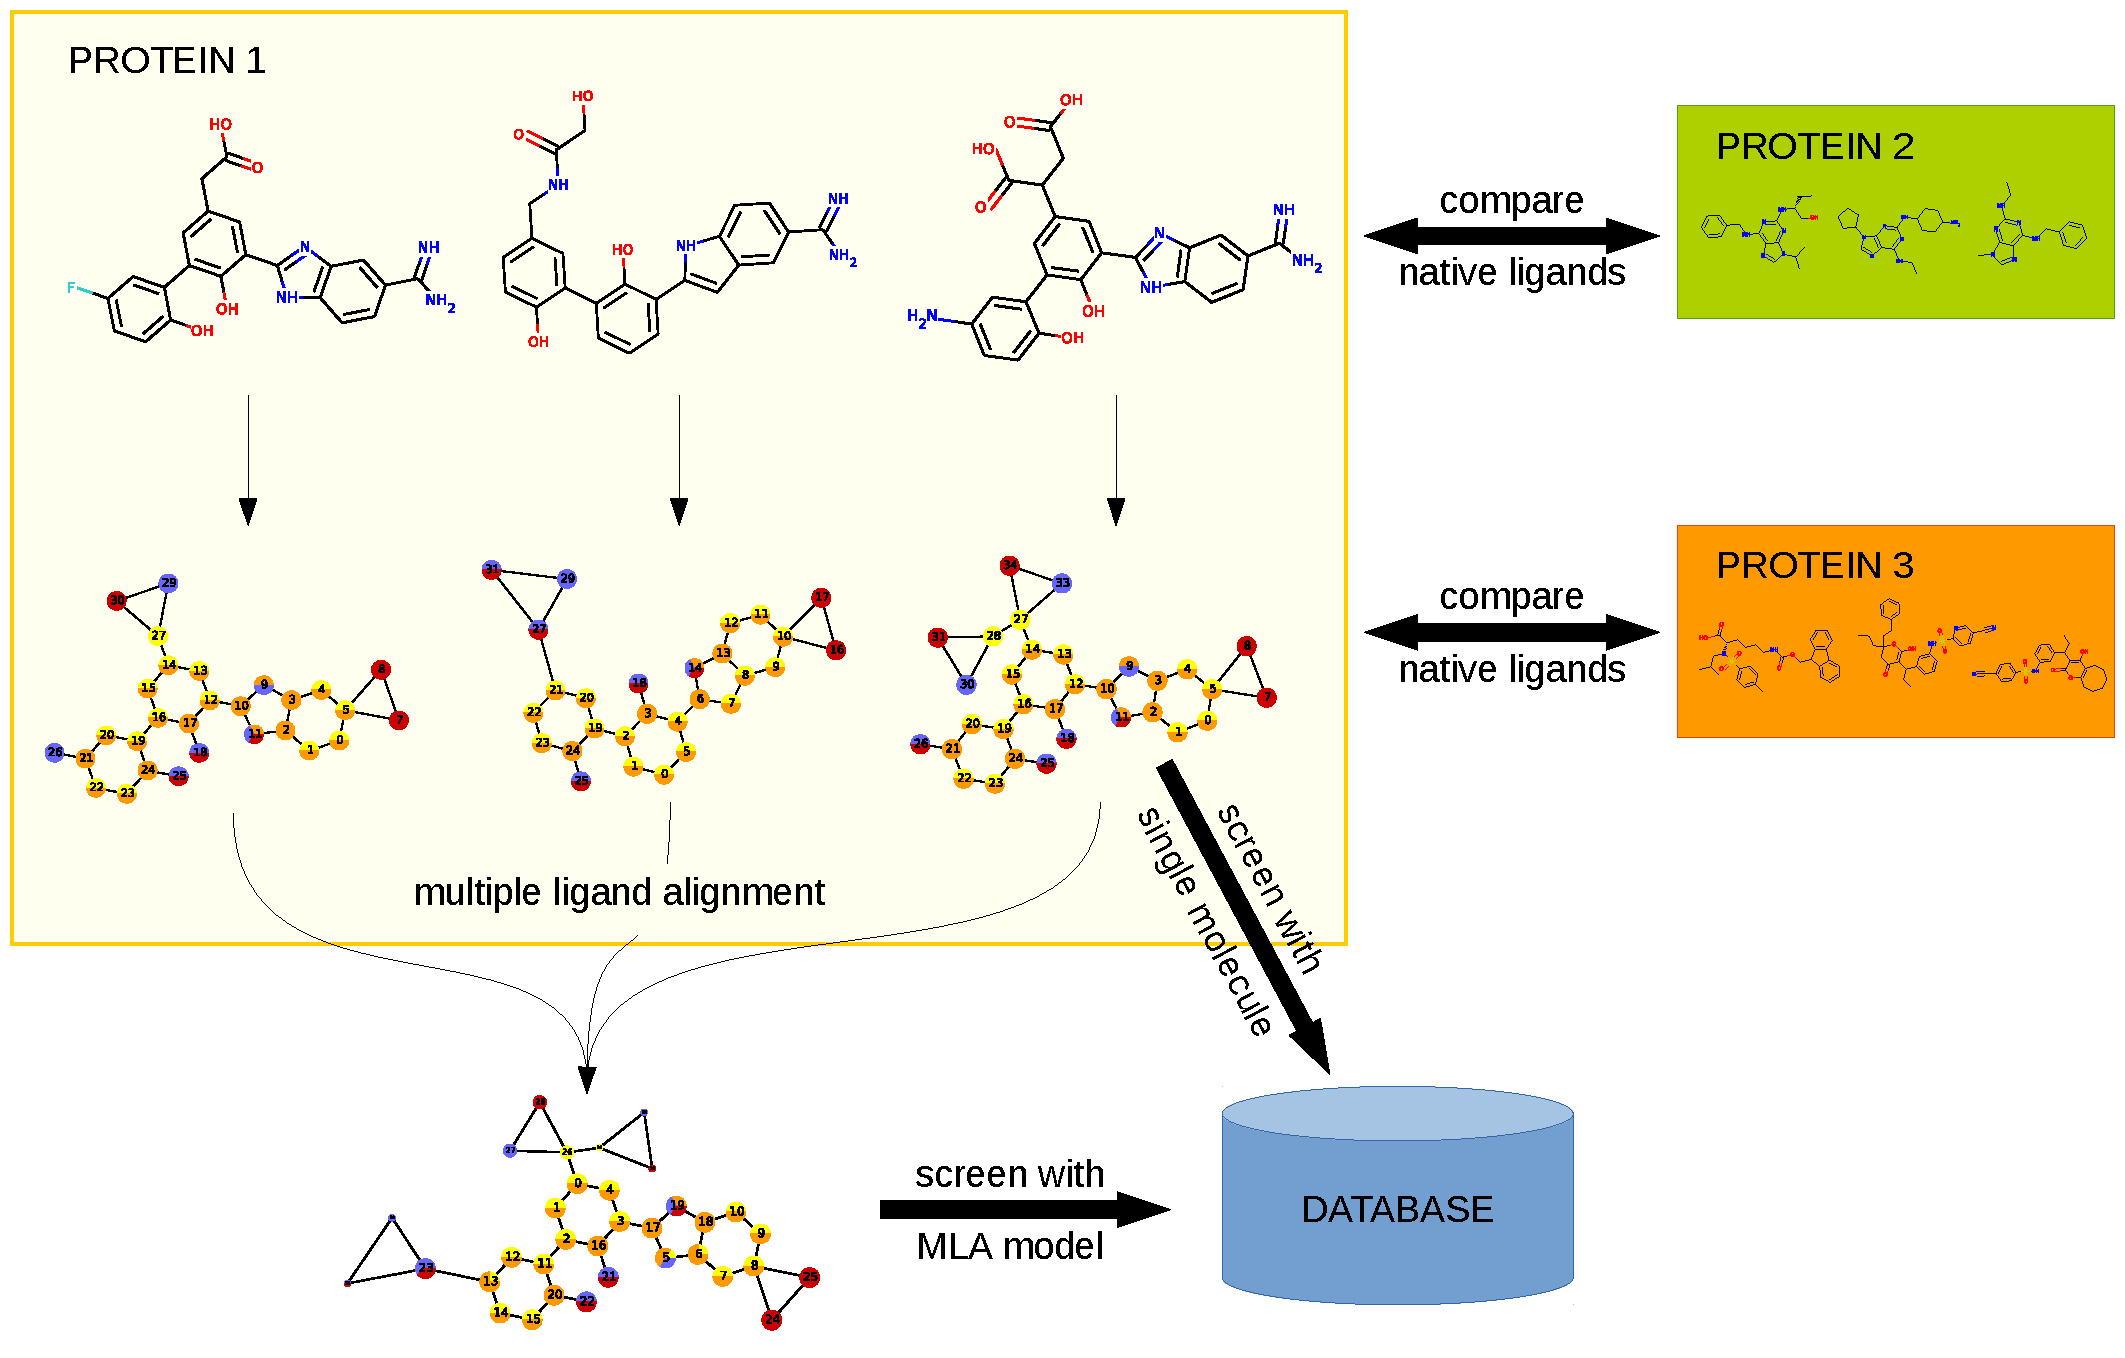
\includegraphics[width=0.85\linewidth]{screen}
%\end{center}
}


\headerbox{5. Results}{name=results,span=2,column=1,below=examples}{ % To reduce this block to 1 column width, remove 'span=2'



%\begin{wrapfigure}{l}{\textwidt}
%    \includegraphics[width=0.7\linewidth]{figures/aug_hack_example1}
%\end{wrapfigure}



 We tested DeCAF in 35 case studies taken from the DUD-E database, to evaluate its power to discriminate between active and inactive molecules.
 We used DeCAF as a classifier and compared it to the SEA (Similarity Ensemble Approach) algorithm \cite{keiser2007relating}.
 To compare sets of ligands, we adapted the approach used in SEA, replacing Tc by DCAF.
 We prepared datasets as shown in the left diagram.
 Then, we tested both classifiers calculating ROC AUC values for every target (below).
%We tested DeCAF in 35 diverse targets taken from the DUD-E database, to evaluate its power to classify molecules as active or inactive.
%We compared DeCAF to the renowned \textbf{SEA (Similarity Ensemble Approach)} algorithm \cite{keiser2007relating}, which uses Tc as a similarity measure.
%Dataset preparation steps are shown on the left diagram.
%Comparison results (\textbf{ROC AUC} values for each receptor) are shown below.
% Please ask me about details.

%\hspace{0pt}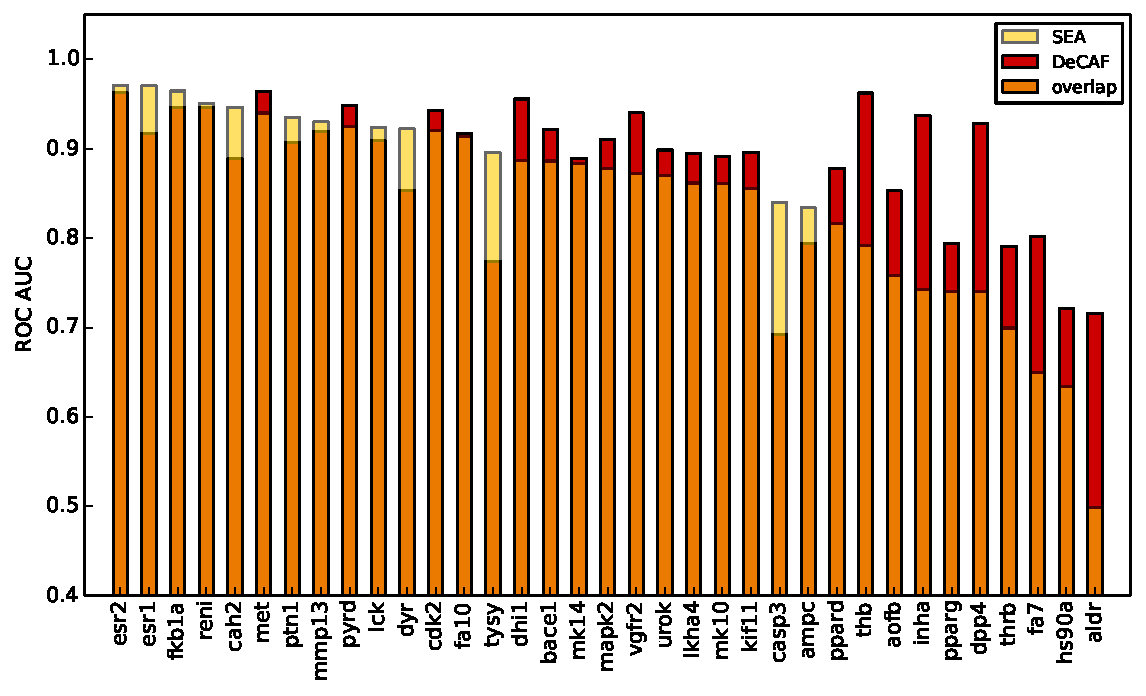
\includegraphics[width=0.95\linewidth]{res}

}


\headerbox{6. Conclusions}{name=conclusion,column=1,below=results,span=2,above=bottom}{
% DeCAF is a chemoinformatical tool that can be helpful in ligand-based drug design.
% It provides a comprehensive molecule description and a fast algorithms for comparing and aligning multiple ligands.
%We proved that DeCAF is a significant improvement over the SEA algorithm, a popular method for comparing sets of ligands.
%\begin{boenumerate}\compresslist
%    \item DeCAF gives better results for 23 out of 35 receptors.
%    \item For targets with easily separable active and inactive datasets, SEA and DeCAF give similar results.
%    \item In cases in which SEA fails to identify active molecules, our method performs substantially better.
%\end{boenumerate}
% It can be also used in other [procedures], such as database screening or drug repositioning.
% DeCAF is written in Python and freely available at \textbf{\color{darkgreen}http://bitbucket.org/marta-sd/decaf}. 
}


\headerbox{7. References}{name=references,column=0,span=1,below=training,above=bottom}{


%\small % Reduce the font size in this block
\renewcommand{\section}[2]{\vskip 0.05em} % Get rid of the default "References" section title
%\nocite{*} % Insert publications even if they are not cited in the poster


%\bibliographystyle{unsrt}
%\bibliography{poster} % Use sample.bib as the bibliography file
}

\end{poster}

\end{document}
